\chapter{Fundamentos tecnológicos}
\label{chap:fundamentos_tecnologicos}

\section{Estado del arte}
\label{sec:estado_arte}

En el ámbito de la robótica autónoma y la utilización de modelos de mundo y utilidad ya existen 
algunos trabajos que tocan estos puntos. A continuación, comentamos brevemente algunos de ellos:

\begin{itemize}
  \item \textbf{e-MDB: a cognitive architecture for lifelong open-ended learning autonomy in robotic systems}~\cite{romero2022mdb}: 
  Tesis doctoral desarrollada por Alejandro Romero Montero que busca diseñar robots que puedan ser útiles 
  en entornos complejos y cambiantes. Para esto, deben ser capaces de realizar tareas en dominios 
  desconocidos a priori (open-ended) y reutilizar el conocimiento y aprender a lo largo de toda 
  su vida (lifelong-learning). Para esto, propone el diseño de sistemas con autonomía de aprendizaje 
  abierto a lo largo de la vida (lifelong open-ended learning autonomy, LOLA). En la tesis, explica 
  la creación de una arquitectura prototipo llamada epistemic Multilevel Darwinist Brain (e-MDB), 
  compuesta por un sistema motivacional y una memoria asociativa a largo plazo (LTM), que es capaz 
  de operar en entornos LOLA. 
  Como mención, comentar que este trabajo es la continuación del MDB\cite{bellas2010multilevel}, cuya principal 
  diferencia con este es el añadido de una memoria episódica, la cual, actúa como almacenamiento para los 
  episodios (conjuntos de percepciones y acciones) y permite el aprendizaje de los distintos modelos, políticas y funciones de representación.
  En relación con el trabajo desarrollado aquí, implementa la utilización de modelos de mundo y 
  de utilidad para representar el comportamiento del robot en el entorno y para proporcionar el valor 
  de utilidad esperado para un estado perceptual determinado, respectivamente.
  
  \item \textbf{Learning adaptable utility models for morphological diversity}~\cite{campos2024learning}: 
  Este trabajo estudia la implementación de enfoques de aprendizaje abierto (open-ended learning) 
  en el campo de la robótica modular. El objetivo es proporcionar la capacidad a estos robots de 
  aprender de forma autónoma modelos de utilidad específicos para cada morfología y que sean 
  capaces de descubrir por sí mismos sus metas. Para esto, presentan un sistema que incorpora 
  motivaciones intrínsecas basadas en la novedad, e introducen una nueva motivación basada en 
  la frustración para tratar de evitar el estancamiento durante la fase de exploración para la recolección 
  de datos de entrenamiento. Este artículo, como el anterior, aborda el aprendizaje de modelos de mundo, 
  que además permiten al robot descubrir su propia morfología, y de modelos de utilidad.

  \item \textbf{A Walk in the Park: Learning to Walk in 20 Minutes With Model-Free Reinforcement Learning}~\cite{smith2022walk}:
  En este proyecto se muestra como un robot cuadrupedo (en concreto un Unitree A1\cite{UnitreeA1dWeb}) aprende a moverse en el mundo real en 
  aproximadamente 20 minutos utilizando aprendizaje por refuerzo profundo libre de modelos. En esta investigación, descartan la 
  implementación del sistema en un entorno simulado a favor de trabajar directamente en entornos reales. Este entorno está 
  formado por terrenos, tanto interiores como exteriores, que han demostrado ser desafiantes para los controladores basados 
  en modelos. Trabajan con acciones a bajo nivel y para lograr el entrenamiento del sistema combinan algoritmos \gls{off-policy} tipo 
  \Gls{sac} con una implementación de \Gls{jac}+\Gls{jit} y un diseño de \Gls{mdp} (estado, acciones, recompensas y resets). Con 
  todo esto, el robot es capaz de aprender un patrón de marcha consistente permitiéndole moverse en todos los terrenos en los que 
  fue entrenado.
  Este trabajo destaca la posibilidad de entrenar modelos consistentes directamente en entornos reales sin pasar por un entorno 
  simulado, concretamente un modelo cuadrupedo de la misma marca que se utilizara en este proyecto.
  \item \textbf{DayDreamer: World Models for Physical Robot Learning}~\cite{wu2023daydreamer}: 
  En este trabajo se trata la utilización de modelos de mundo tipo Dreamer (modelo de mundo tradicional + planificación en “imaginación”) 
  para realizar aprendizaje por refuerzo directamente en robots reales. Esta técnica permite reducir el “prueba y error” que 
  normalmente necesita un modelo para aprender a moverse por el mundo y sustituirlo por el algoritmo Dreamer, que permite 
  continuar aprendiendo a partir de un modelo de mundo previamente entrenado. Este sistema fue aplicado en 4 robots diferentes 
  con los mismos hiperparametros y proporciona mejores resultados en menos tiempo que otras aproximaciones como los sistemas 
  libres de modelos. Entre los robots utilizados hay un cuadrupedo Unitree A1 que, con este modelo, es 
  capaz de aprender a darse la vuelta desde su espalda, ponerse de pie y caminar en aproximadamente 1 hora. Además, aprendio a 
  resistir empujones y darse la vuelta en 10 minutos.
  \item \textbf{Recurrent World Models Facilitate Policy Evolution}~\cite{ha2018recurrent}: 
  Este proyecto estudia la implementación de una nueva arquitectura en la que el agente aprende un modelo de mundo de manera 
  no supervisada a partir de las observaciones y las acciones, para después entrenar una política simple usando estas 
  representaciones comprimidas. 
  En concreto, la propuesta divide al agente en tres módulos: un codificador visual que comprime la imagen en un espacio 
  latente (una representación comprimida de la información del entorno, describe este entorno que percibe el agente de manera simplificada) \( z_t \), 
  un modelo recurrente predictivo, que es el encargado de predecir el siguiente estado latente \( z_{t+1} \), y un controlador 
  compacto y simple. Esto permite obtener un controlador simple que facilita la optimización mediante técnicas evolutivas.
  Además, explora el entrenamiento de una política dentro del propio modelo de mundo, en lugar de hacerlo en un entorno real.
  Este proyecto sienta las bases para trabajos posteriores como el antes mencionado DayDreamer.
\end{itemize}


\section{Tecnologías empleadas}
\label{sec:tecnologias_empleadas}

Con el fin de facilitar la explicación de las distintas tecnologías empleadas en el desarrollo de este 
proyecto, las dividiremos en bloques o “entornos” que se describirán a continuación:


\subsection{Entorno Python}
\label{sec:entorno_python}

Python\cite{PythonWeb} es un lenguaje de programación \gls{interpretado}, multiplataforma, de propósito general 
y de alto nivel, conocido por su sencillez y sintaxis clara (fácilmente legible). 
Es ampliamente utilizado para numerosos ámbitos de desarrollo, entre los cuales se encuentran: el desarrollo software, 
data science, desarrollo web y aprendizaje automático, entre otros.
Cuenta con un enorme ecosistema de bibliotecas, lo que amplía en gran medida sus capacidades y lo convierte en uno de los 
lenguajes más utilizados en la actualidad.

Python fue el lenguaje de programación principal en el desarrollo de este proyecto, junto con las siguiente 
librerías:


\begin{itemize}
  \item \textbf{sys}~: La librería sys es un módulo estándar de Python y proporciona acceso a variables y a funciones del 
  intérprete. Su función es interactuar con el entorno de ejecución del lenguaje y con el intérprete, además de utilizarse 
  para obtener los argumentos con los que se ejecutó el programa, terminar el programa con el código de salida, interactuar 
  con la entrada y salida, etc.

  \item \textbf{time}~: La librería time es un módulo estándar de Python que da acceso a funciones relacionadas 
  con el tiempo como por ejemplo: pausar el programa, medir duraciones, obtener marcas de tiempo, etc. 
  
  \item \textbf{os}~: La librería os es un módulo estándar de Python que permite la interacción con el sistema 
  operativo. Sirve para trabajar con rutas, variables de entorno y archivos, además de poder ejecutar operaciones a nivel de sistema.
  
  \item \textbf{random}~: La librería random es un módulo estándar de Python utilizada para generar números 
  pseudoaleatorios y realizar operaciones típicas de muestreo cómo seleccionar elementos al azar, barajar listas, etc.
  
  \item \textbf{pickle}~: La librería pickle es un módulo estándar de Python que sirve para serializar 
  y deserializar objetos, es decir, permite convertir objetos como listas o diccionarios, a una secuencia de bytes para guardarlo 
  en un archivo y realizar la operación inversa.
  
  \item \textbf{numpy}~\cite{NumpyWeb}: La librería numpy es un proyecto de código abierto que permite la computación 
  numérica en Python proporcionando estructuras y funciones eficientes. Es ampliamente utilizado para trabajar con 
  matrices y vectores, realizar operaciones matemáticas vectorizadas y también es usada para álgebra, estadística y generación de 
  datos. Además, sirve de base para muchas otras librerías como pandas y scikit-learn.
  
  \item \textbf{matplotlib}~\cite{MatplotlibWeb}: Es una librería de Python usada para la visualización y el 
  análisis de datos, que permite crear gráficas en 2D y 3D. Posibilita una alta personalización tanto del formato como de la 
  propia gráfica y su forma de representar los datos. 
  En concreto para este proyecto utilizamos el módulo matplotlib.pyplot que ofrece una interfaz similar a Matlab.

  \item \textbf{TensorFlow}~\cite{TensorflowWeb}: Framework de código abierto para aprendizaje automático y \Gls{deep learning} 
  desarrollado por Google\cite{GoogleWeb}. Utilizada para entrenar y evaluar modelos basados en redes neuronales, que son 
  ejecutados de manera eficiente tanto en GPU como en CPU. 
  Sus usos principales son la construcción de redes neuronales, el \Gls{deep learning}, producción y despliegue con herramientas como 
  TensorFlow Lite y monitorización del entrenamiento con TensorBoard.

  Para este trabajo se utilizó Keras\cite{KerasWeb}, un \Gls{api} de alto nivel incluido en TensorFlow que permite crear y entrenar 
  redes neuronales de manera sencilla, además de incluir una amplia gama de modificaciones que trataremos más profundamente en partes 
  posteriores de la memoria (sección \ref{chap:desarrollo}, página \pageref{chap:desarrollo}).
\end{itemize}


\subsection{Entorno Optitrack}
\label{sec:entorno_optitrack}

Optitrack (perteneciente a la empresa NaturalPoint\cite{NaturalPointWeb}) es un sistema de captura de movimiento 
que utiliza cámaras ópticas situadas alrededor de un espacio para registrar el movimiento ocurrido en él. Ampliamente utilizado en 
animación, realidad virtual, robótica e investigación, proporciona métricas precisas y en tiempo real de la posición y la orientación 
de los objetos capturados. 

Comenzaremos explicando los elementos de hardware que conforman este entorno. El sistema hace uso de unas esferas reflectantes llamadas 
marcadores (figura \ref{fig:marker_optitrack}), que permiten a las cámaras captar la posición de estos marcadores en el espacio. Hay distintas distribuciones, desde trajes de cuerpo completo que permiten 
capturar el movimiento humano (muy utilizado en animación) hasta un único marker para obtener la ubicación de un objeto sencillo. Para 
este proyecto se utilizaron 6 marcadores en total: tres de ellos ubicados en la cabeza del robot y otros tres situados en el objetivo. 
En ambos casos se colocaron en forma de triángulo, con el fin de formar un \gls{markerset}, cuyo concepto explicaremos más adelante, y calcular 
el punto medio de los objetos.



\begin{figure}[hp!]
  \centering
  \includegraphics[width=0.5\textwidth]{imaxes/optitrack/marker_optitrack.png}
  \caption{Marcadores utilizados en el entorno Optitrack.}
  \label{fig:marker_optitrack}
\end{figure}

El componente principal de este sistema son las propias cámaras Optitrack, las cuales emiten una luz infrarroja que 
permite capturar el reflejo de los marcadores para, posteriormente, juntar la información de todas las cámaras utilizadas, obtener la 
posición del objeto y reconstruir la trayectoria descrita por los markers.


Para definir con precisión las especificaciones del proyecto, se emplearon ocho cámaras OptiTrack, en concreto el modelo Primex13W 
(figura \ref{fig:camara_optitrack}). Se situaron en una estructura rack en el techo con la siguiente disposición: una cámara en cada esquina y las cuatro restantes 
centradas en cada una de las paredes (como se puede apreciar en las figuras \ref{fig:esquema_estructura} y \ref{fig:Estructura_camaras_optitrack}). Se optó por esta distribución 
al considerarse la más adecuada para adaptarse al entorno de trabajo y capturar de forma completa el espacio de movimiento del robot.
Cabe destacar que al comienzo de este proyecto solo se contaba con 4 cámaras, situadas en la parte central de cada lado del rack. Con esta distribución, 
si bien era posible llevar a cabo el proyecto, lo limitaba en gran medida debido a que ocasionaba que las cámaras perdieran la posición del robot al 
no haber suficientes (el mínimo recomendado son tres viendo cada marcador) de ellas que pudieran seguirlo en ciertas zonas del espacio. 

\begin{figure}[hp!]
  \centering
  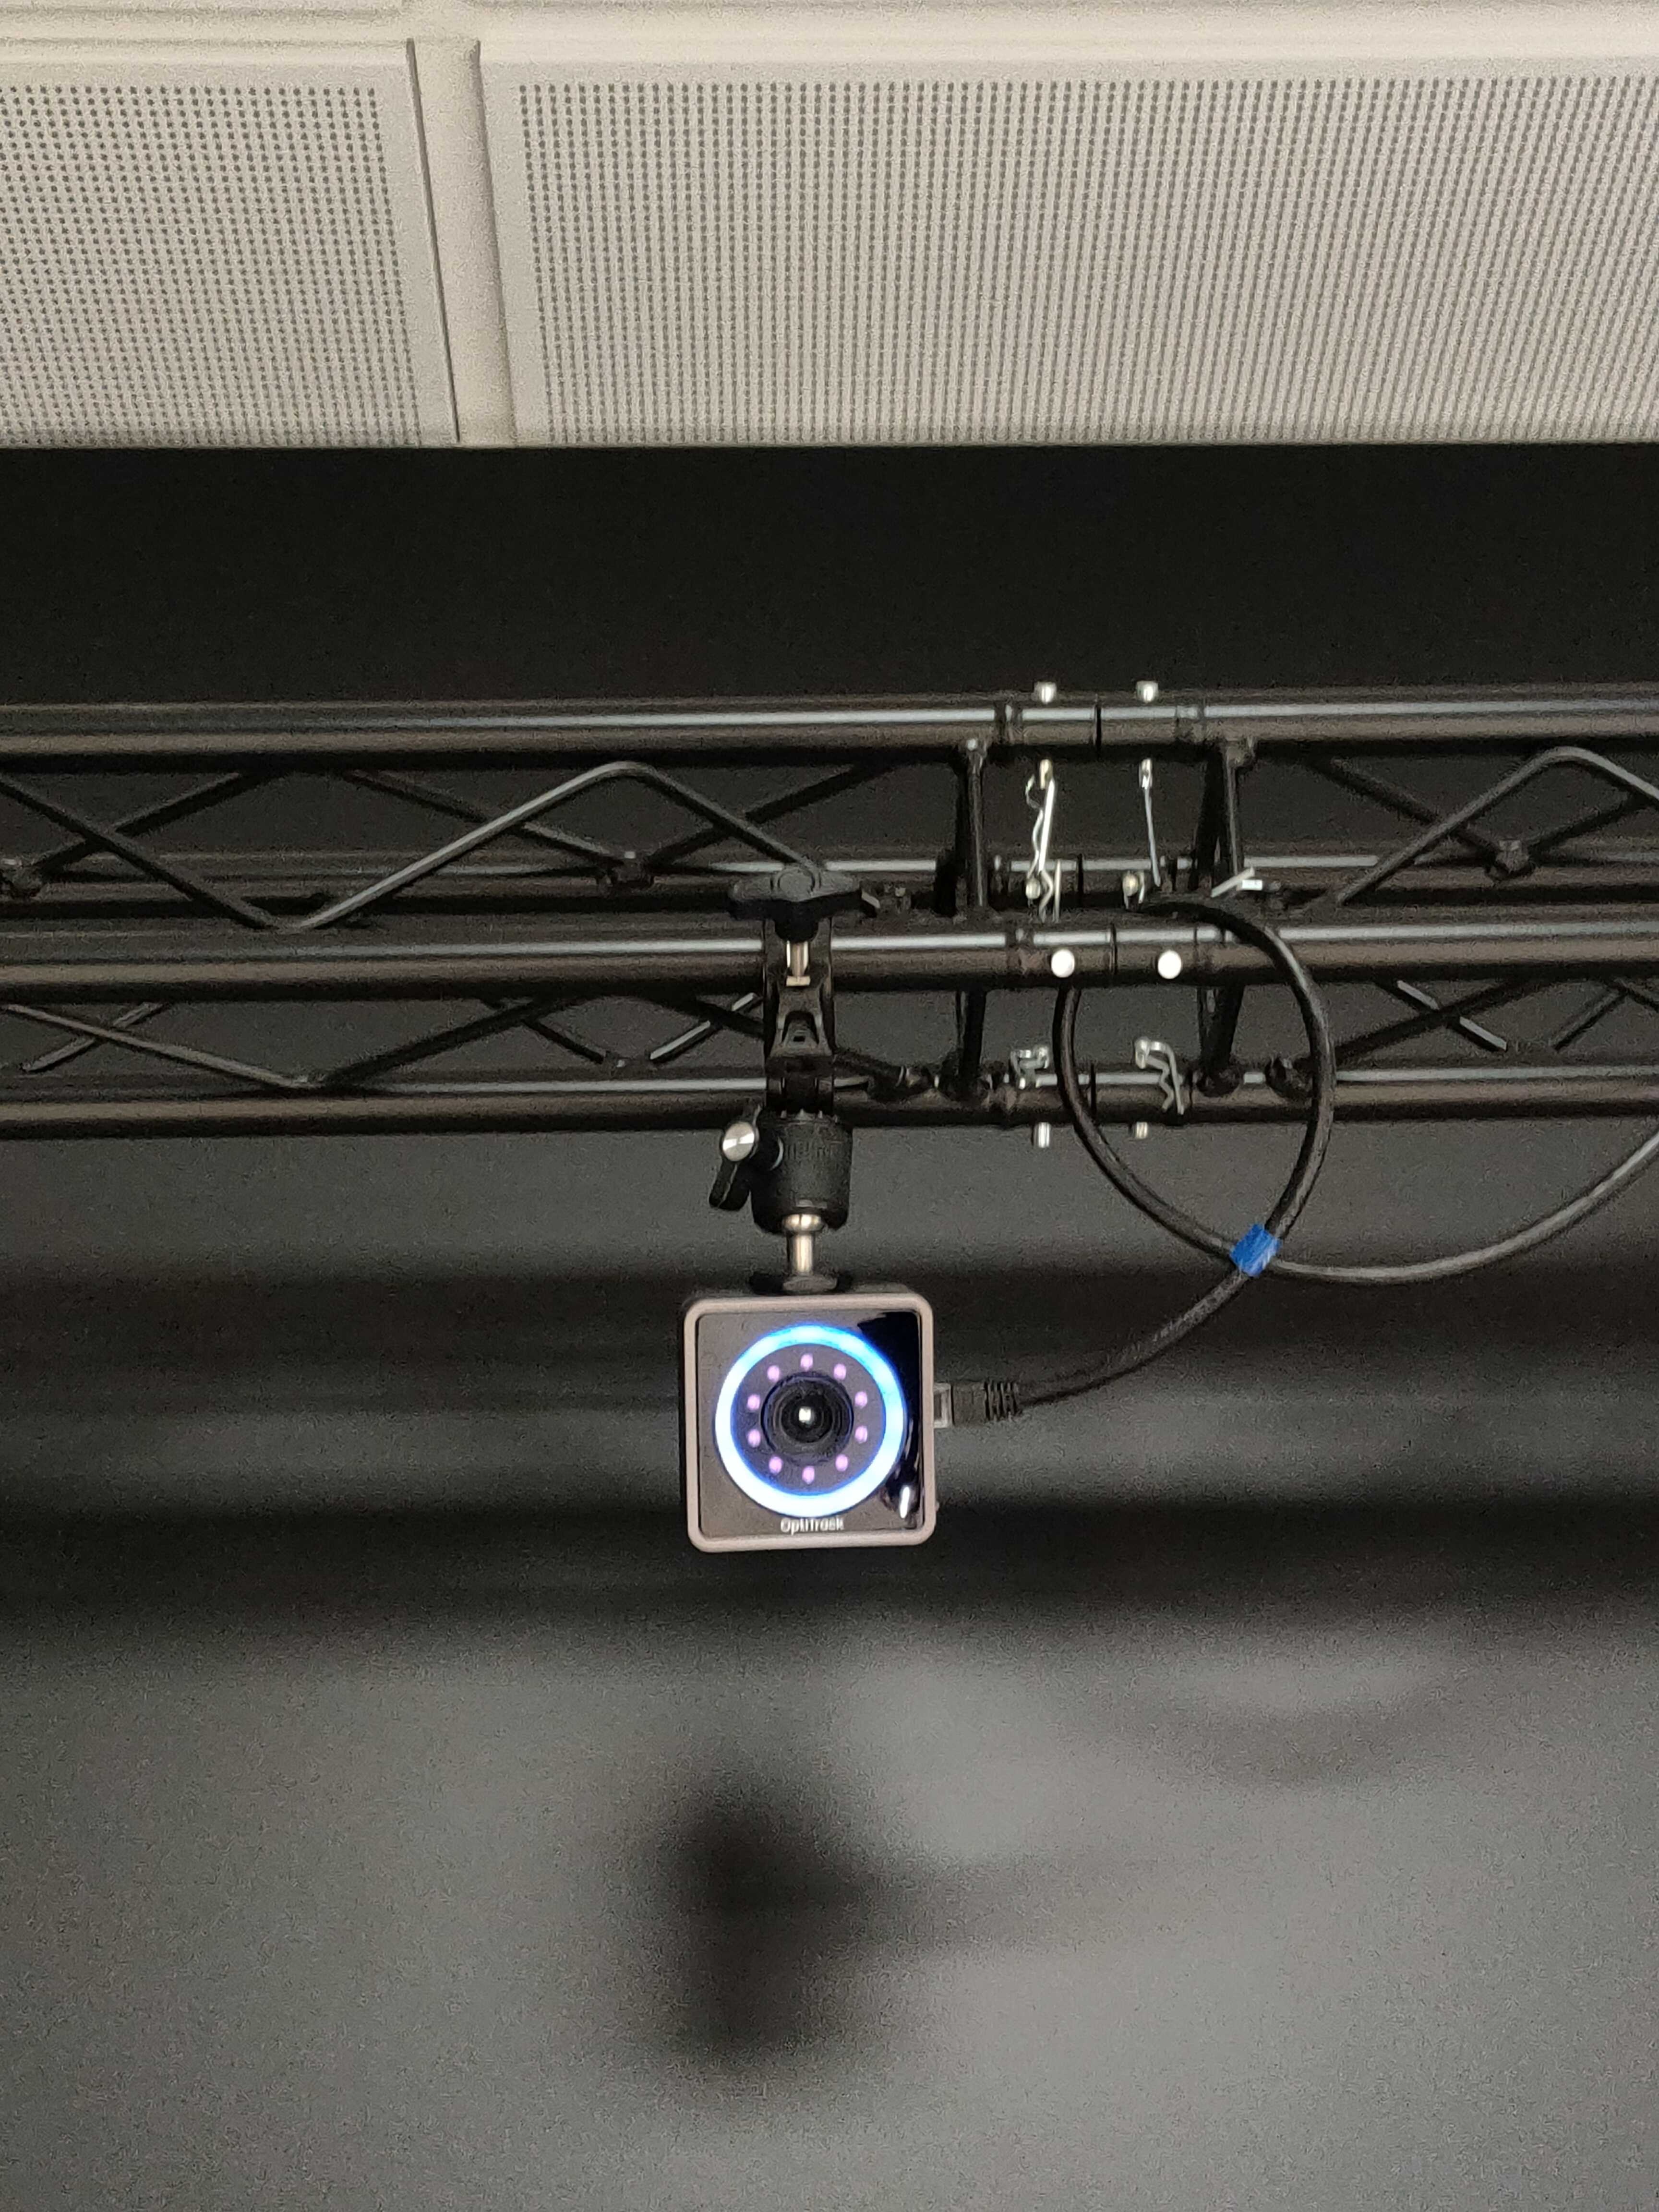
\includegraphics[width=0.5\textwidth]{imaxes/optitrack/camara_optitrack.png}
  \caption{Cámaras Primex13W utilizadas en el entorno Optitrack.}
  \label{fig:camara_optitrack}
\end{figure}

\begin{figure}[hp!]
  \centering
  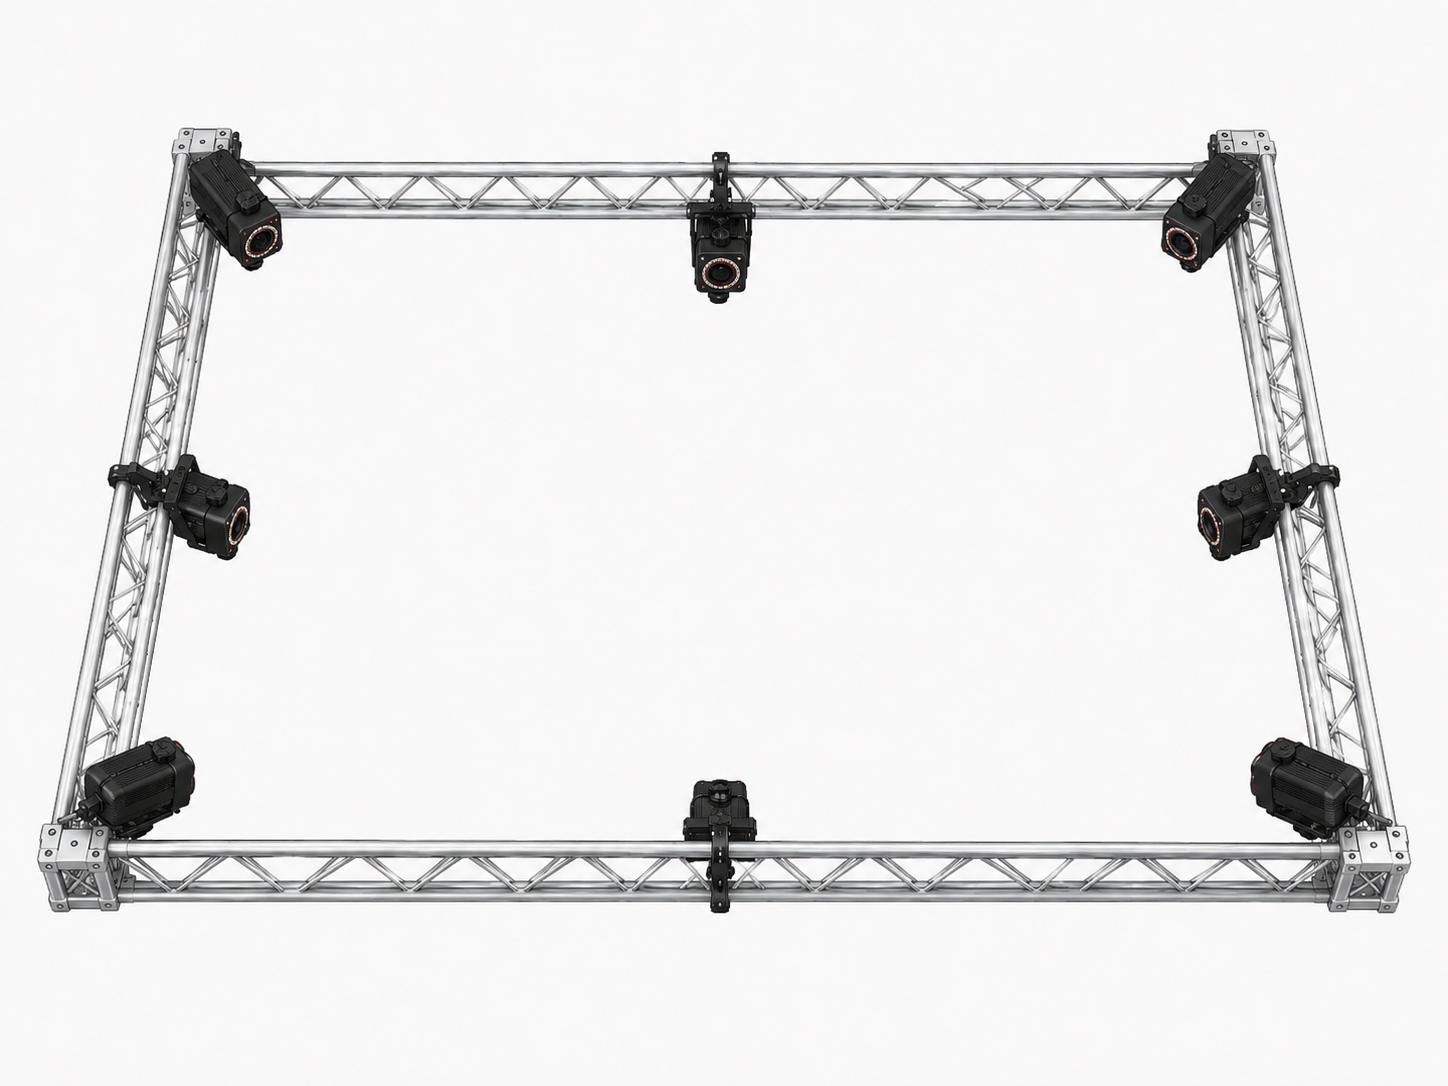
\includegraphics[width=0.5\textwidth]{imaxes/optitrack/estructura_camaras_optitrack.png}
  \caption{Esquema de la estructura de las cámaras Optitrack.}
  \label{fig:esquema_estructura}
\end{figure}

\begin{figure}[hp!]
  \centering
  \begin{subfigure}[c]{0.3\textwidth}
    \includegraphics[width=\textwidth]{imaxes/optitrack/estructura_cam1.png}
    \caption{Parte 1.}
    \label{fig:Estructura_camaras_optitrack_1}
  \end{subfigure}
  \hspace{0.1\textwidth}
  \begin{subfigure}[c]{0.3\textwidth}
    \includegraphics[width=\textwidth,height=3cm]{imaxes/optitrack/estructura_cam2.png}
    \caption{Parte 2.}
    \label{fig:Estructura_camaras_optitrack_2}
  \end{subfigure}
  \caption{Estructura de las cámaras Optitrack.}
  \label{fig:Estructura_camaras_optitrack}
\end{figure}

Para recibir la información de las cámaras y ejecutar Motive\cite{MotiveWeb} (el software para procesar la información y trabajar con ella) 
se requería un equipo conectado a la red de las cámaras. Para esto se utilizó un Intel NUC con Windows 11 con la versión (3.3.4.1) 
del Motive instalado.

La conectividad entre las cámaras y el NUC requería que ambos estuvieran conectados a la misma red para poder transmitir la información, para 
ello se utilizó un Switch, al cual se conectan los dispositivos vía Ethernet. Además, el NUC estaba conectado por WiFi a la red del centro 
para poder transmitir los datos obtenidos (mediante paquetes \Gls{udp}) al ordenador del estudiante, instalado con Linux,  para poder procesar y 
utilizar los datos posteriormente.

Una vez explicado la parte de hardware referente a este entorno, pasaremos a tratar el software necesario para el desarrollo de este proyecto. 
Motive es el software de Optitrack encargado de controlar el sistema de captura de movimiento, a través de él 
se puede configurar el entorno y transmitir los datos a otros equipos, además de guardarlos para su posterior uso. 
En su pantalla principal (figura \ref{fig:interfaz_motive}) se puede observar la colocación de las cámaras así como el espacio que capturan y los objetos dentro de este en tiempo 
real. En los distintos apartados se puede configurar las propiedades de los objetos, crear \gls{markerset} y \gls{rigidbody} o modificar los ajustes de las 
cámaras, entre otras opciones.

\begin{figure}[hp!]
  \centering
  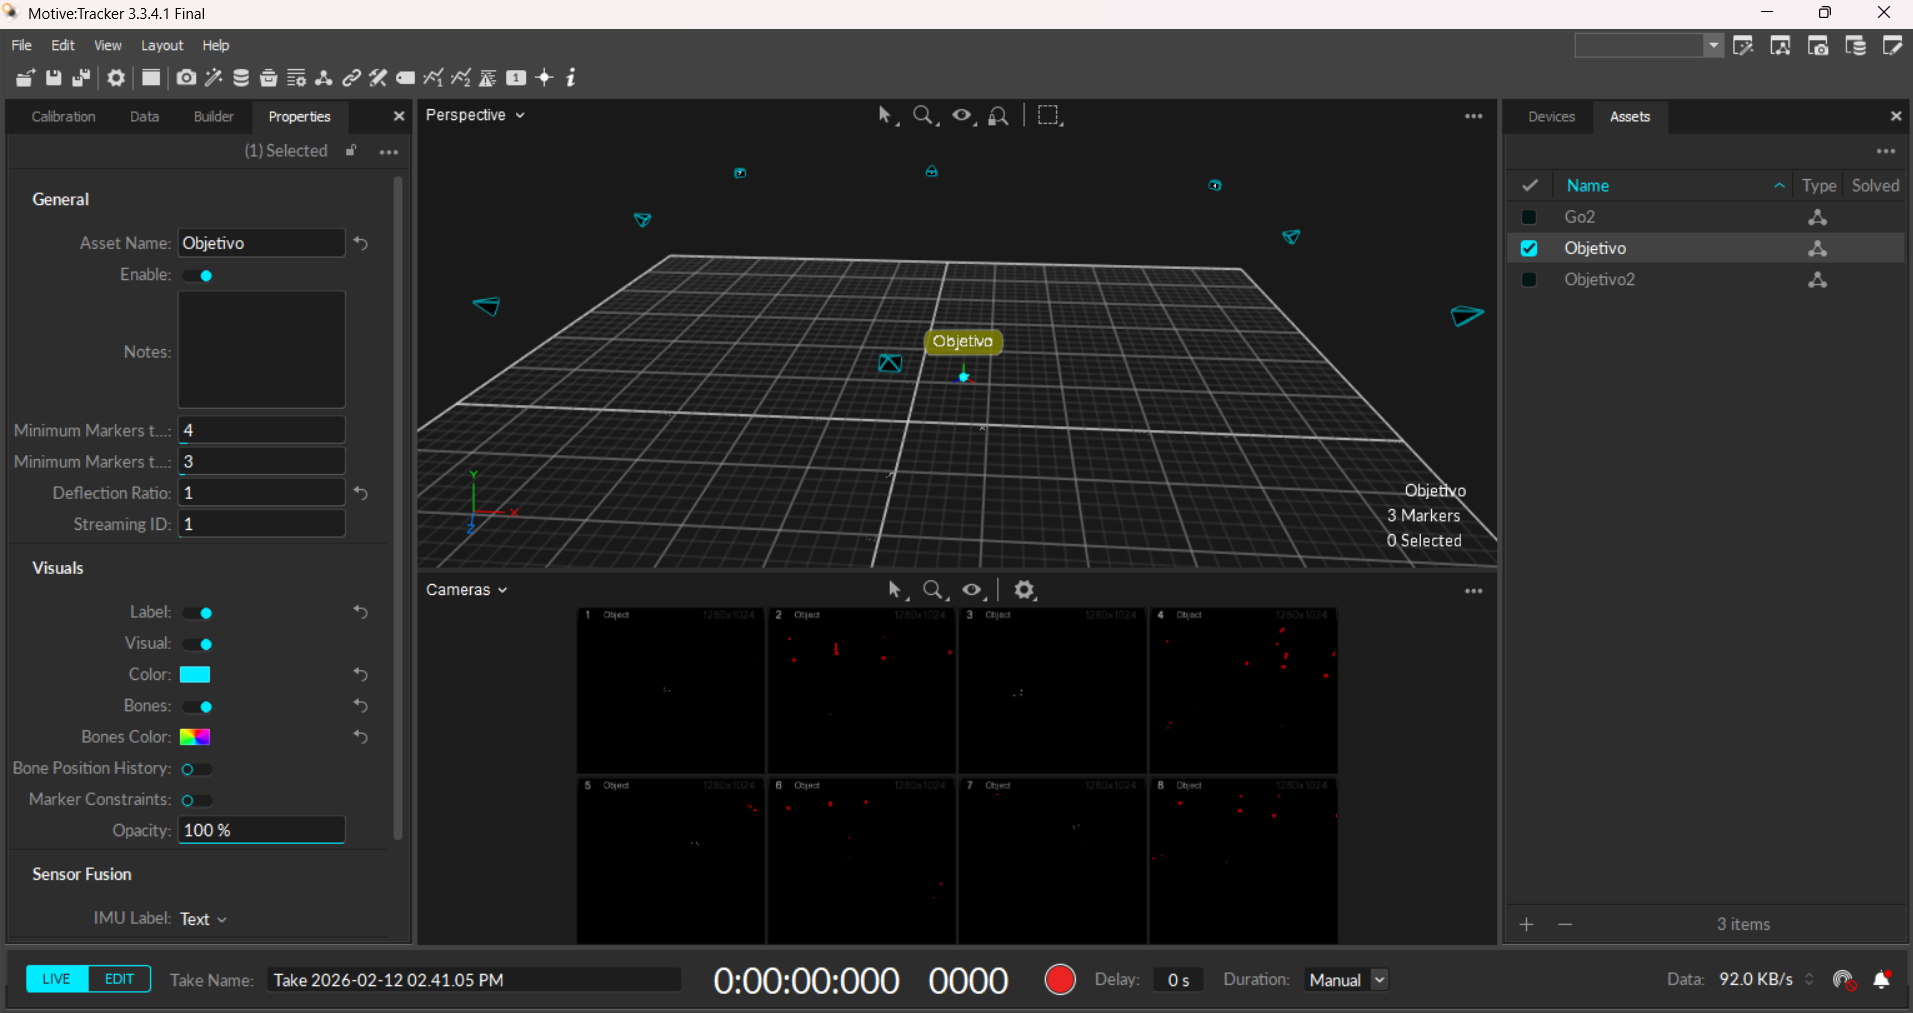
\includegraphics[width=0.75\textwidth]{imaxes/motive/Captura_Interfaz_Motive.png}
  \caption{Interfaz principal del software Motive.}
  \label{fig:interfaz_motive}
\end{figure}

Para utilizar correctamente el sistema Optitrack y el software motriz, lo primero que hay que realizar es la calibración del sistema y del volumen de trabajo en el que 
se va a operar. Para esto, se han seguido las instrucciones disponibles en la documentación del propio programa. Esta calibración consta de dos 
partes tras iniciarla:

\begin{itemize}
  \item En el primer paso se buscará rellenar el volumen de captura (figura \ref{fig:volumen_captura}) que corresponde al campo de visión de las cámaras usando una 
  barra equipada con marcadores (figura \ref{fig:barra_calibracion}). Para lograrlo, se debe recorrer el espacio realizando movimientos en forma de infinitos con 
  la barra, mientras se supervisa el progreso en el programa. En la aplicación, cada cámara mostrará un recuadro que representa el área que está 
  captando. Cada movimiento realizado con la barra dejará un rastro en los recuadros de aquellas cámaras que hayan detectado el gesto. Una vez 
  que se haya cubierto suficiente superficie con estas pasadas, la aplicación lo indicará mostrando un borde verde alrededor de los recuadros, señal 
  de que este paso puede darse por completado.

  \begin{figure}[hp!]
    \centering
    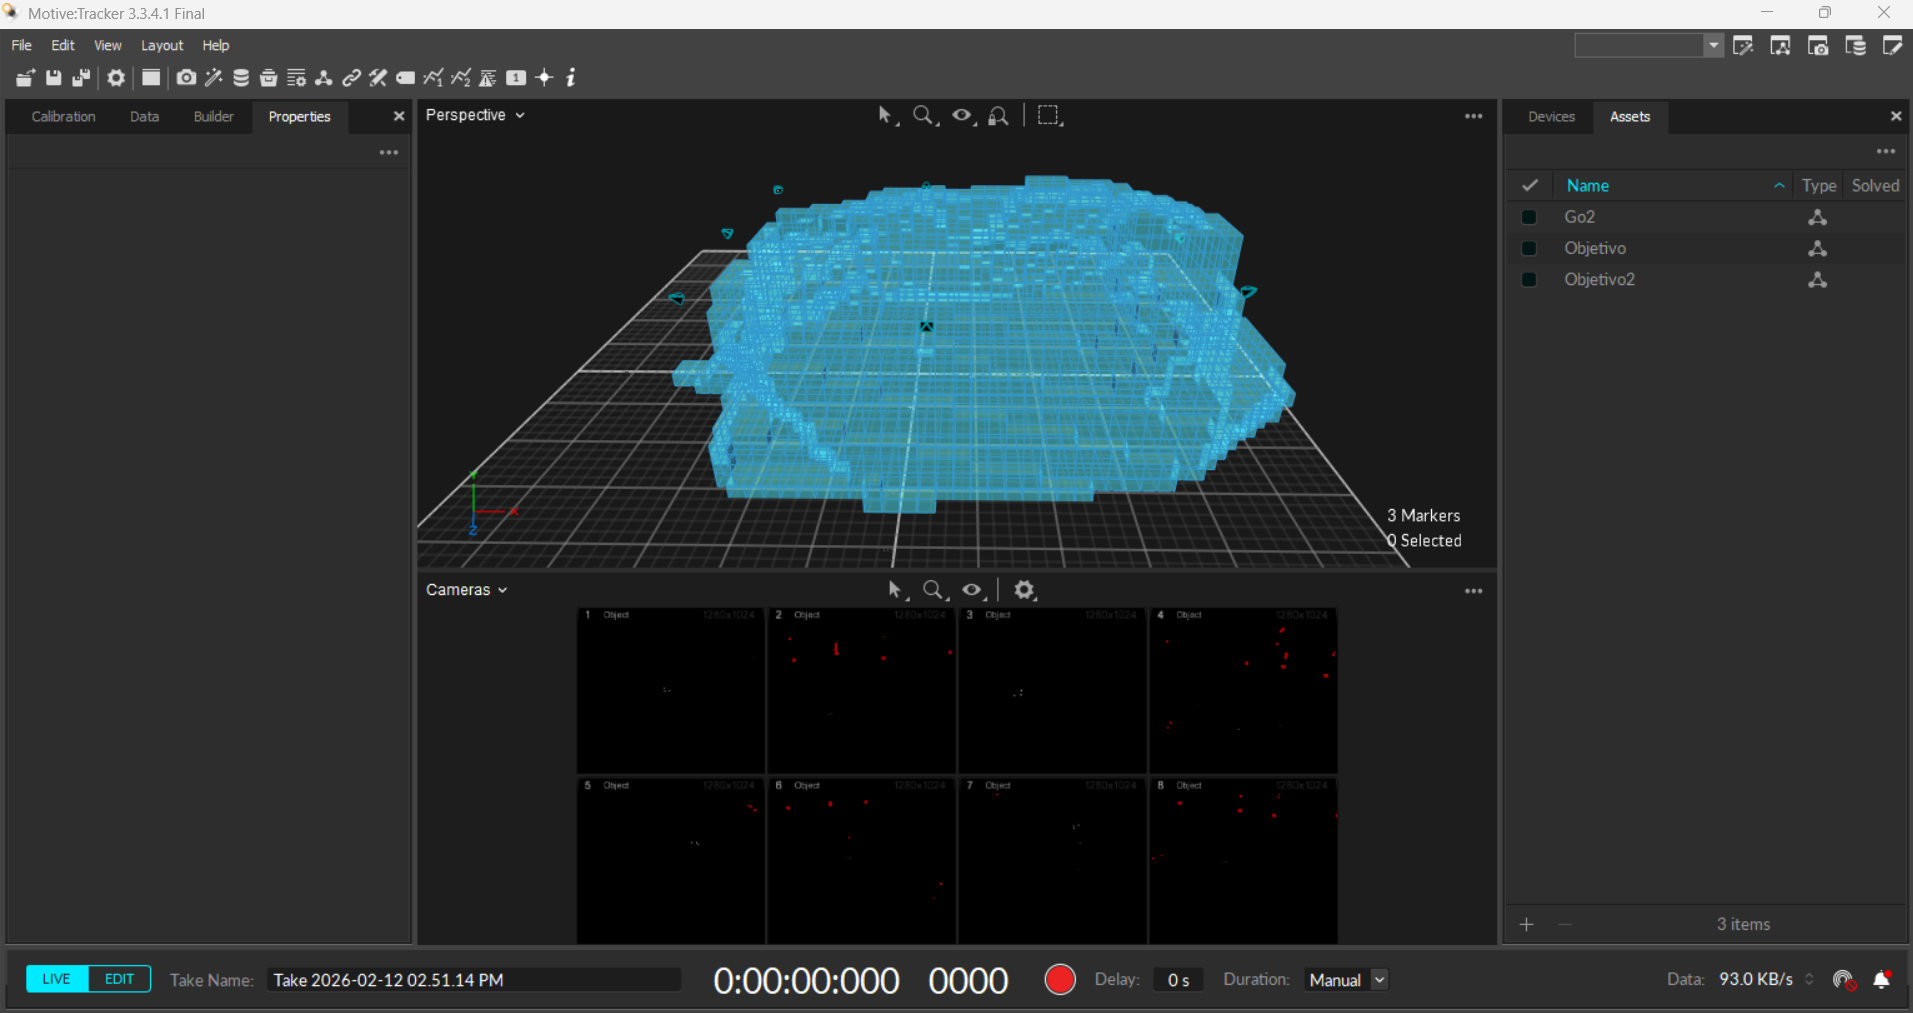
\includegraphics[width=0.75\textwidth]{imaxes/motive/Captura_Volumen_De_Captura.png}
    \caption{Volumen de captura de Motive.}
    \label{fig:volumen_captura}
  \end{figure}

  \begin{figure}[hp!]
    \centering
    \includegraphics[width=0.5\textwidth]{imaxes/optitrack/barra_calibracion.png}
    \caption{Barra de calibración.}
    \label{fig:barra_calibracion}
  \end{figure}

  \item Tras esto, se usará una escuadra (figura \ref{fig:escuadra_calibracion}), también equipada con marcadores, para situar el origen del espacio (el punto [0, 0, 0] del espacio).
  
  \begin{figure}[hp!]
    \centering
    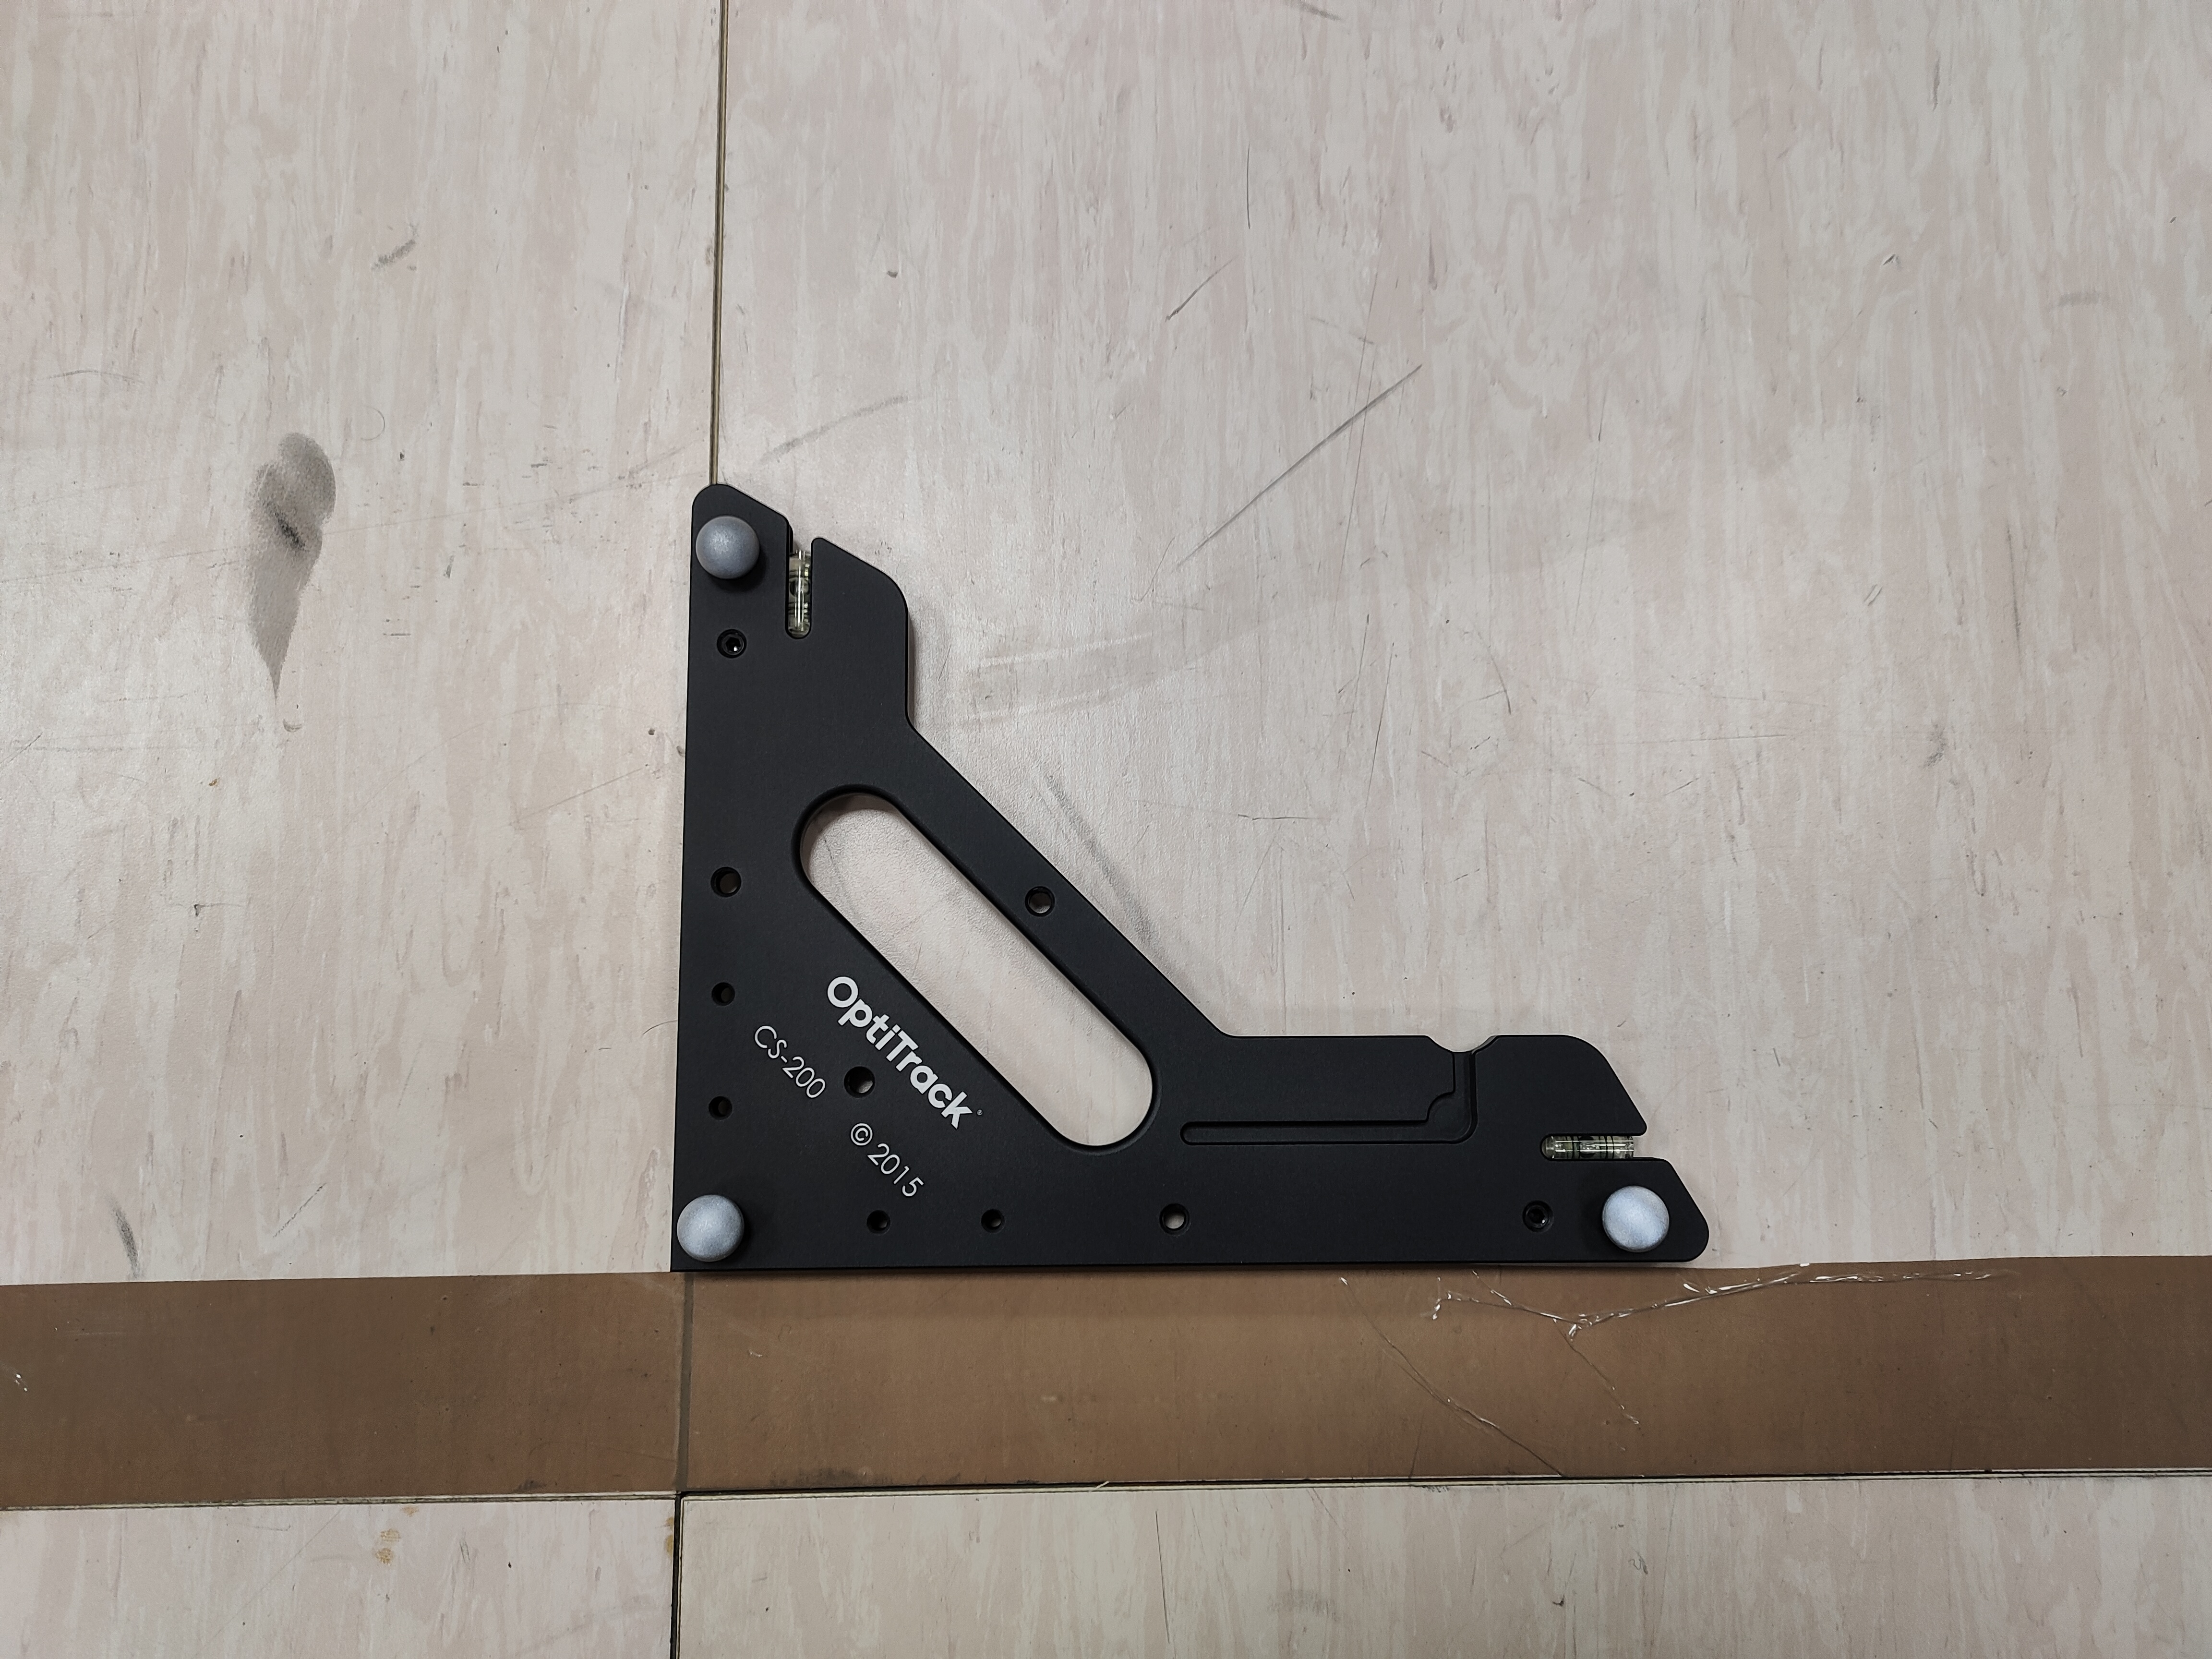
\includegraphics[width=0.5\textwidth]{imaxes/optitrack/escuadra_calibracion.png}
    \caption{Escuadra de calibración.}
    \label{fig:escuadra_calibracion}
  \end{figure}

\end{itemize}

Una vez calibrado el entorno, se podrá comenzar a modificar las distintas opciones disponibles, como por ejemplo, cambiar la frecuencia de muestreo de las cámaras. Para 
este proyecto se han dejado todas las opciones de configuración por defecto (figura \ref{fig:configuracion_motive}) a excepción de las referentes al streaming de datos: se 
habilitó esta opción, se estableció la IP del servidor (el Intel NUC) y se configuró en modo \gls{unicast} (se optó por la utilización de este modo en lugar de multicast 
debió a que este segundo modo presentaba problemas de conexión a la hora de transmitir datos. Además, el modo multicast está pensado para enviar información a lo largo de 
la red a varios ordenadores receptores, sin embargo en nuestro caso concreto solo se utilizará un único receptor, por lo que el modo unicast se adapta perfectamente 
al funcionamiento del sistema).

\begin{figure}[hp!]
  \centering
  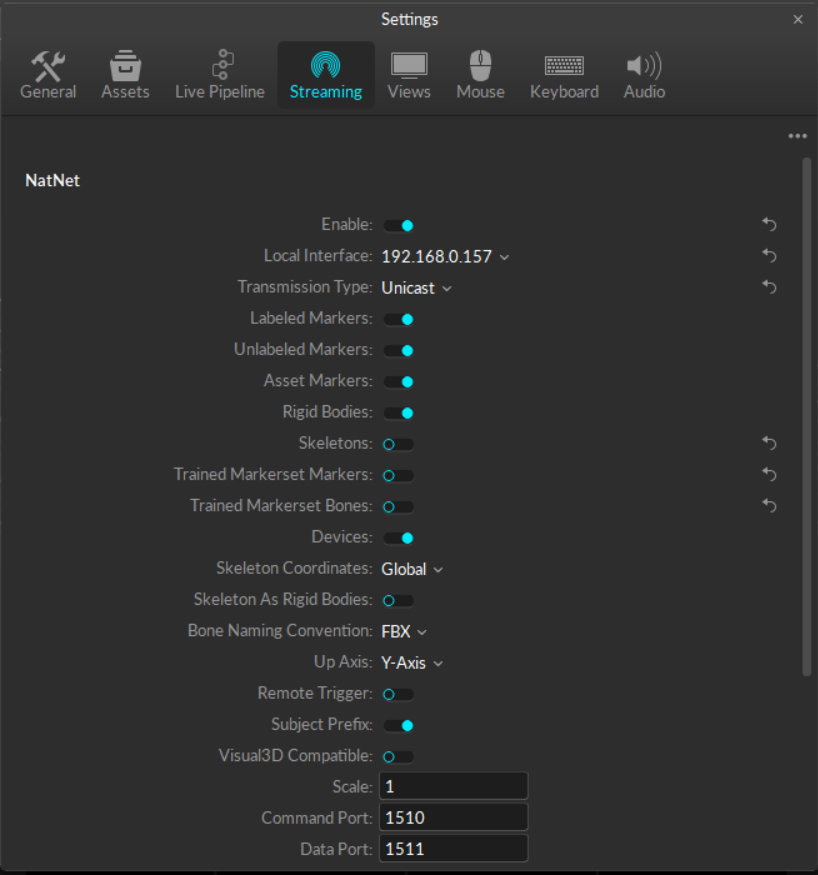
\includegraphics[width=0.75\textwidth]{imaxes/motive/Captura_Configuracion_Streaming.png}
  \caption{Configuracion de Motive.}
  \label{fig:configuracion_motive}
\end{figure}

Tras terminar de configurar el programa, se procedió a la colocación de los marcadores en los objetos y a la creación de los \gls{markerset} para el robot y el 
objetivo, asignándoles los nombres correctos (“Go2” y “Objetivo”) para poder identificarlos en el ordenador con Linux una vez transferidos. 

Para poder recibir estos datos transferidos desde Motive, utilizamos el \Gls{sdk} de NatNet\cite{NatNetSDKWeb} proporcionado por Optitrack. Este 
conjunto de herramientas y librerías proporciona las funciones necesarias para conectarse y recibir la información enviada de manera síncrona por Motive a través 
de la red en el programa que lo requiera, en este caso el programa de Python creado para recopilar los datos del robot para entrenar los 
modelos. Utilizaremos este \Gls{sdk} casi sin modificaciones, excepto por una función que es necesario modificar para filtrar y separar los datos referentes 
al robot y al objetivo (lo cual explicaremos más en detalle en el apartado de Desarrollo, sección \ref{chap:desarrollo}, página \pageref{chap:desarrollo}).


\subsection{Entorno del robot}
\label{sec:entorno_robot}

El robot que se utilizara para este proyecto es el Unitree Go2 (figura \ref{fig:robot_go2}), un cuadrupedo creado por la empresa china Unitree Robotics para proporcionar 
una locomoción dinámica y diseñado para educación, investigación e industria. Cuenta con varios modelos disponibles (con precios que oscilan entre los 1.600\$ y los 14.500\$ para la 
opción más completa), en concreto el CITIC (Centro de Investigación en Tecnologías de la Información y las Comunicaciones) cuenta con el modelo EDU PLUS. Está pensado para moverse en 
entornos reales por su gran movilidad y estabilidad debida a su forma cuadrúpeda y a sus sensores integrados; cuenta con cámaras, un \Gls{lidar}, sensores en las patas para detectar el 
contacto con el suelo y una \Gls{imu}. Además cuenta con computación propia para controlar estas capacidades y conectividad WiFi/Ethernet y Bluetooth. Gracias a estas tecnologías es posible 
controlarlo con un mando o con el propio teléfono para que se mueva y ordenarle comandos e instrucciones con las que viene preprogramado.

\begin{figure}[hp!]
  \centering
  \includegraphics[width=0.5\textwidth]{imaxes/RobotGo2.png}
  \caption{Robot Unitree Go2.}
  \label{fig:robot_go2}
\end{figure}

Además de las funciones con las que viene programado por defecto, es posible conectarlo a un ordenador vía Ethernet (al momento de realizar este trabajo esta es la única 
manera de poder enviarle instrucciones por código desde un ordenador) para controlarlo y enviarle comandos. Para esto utilizaremos el \Gls{sdk}\cite{UnitreeGo2Doc} 
que proporciona Unitree en su GitHub\cite{UnitreeGo2PythonSDK}, concretamente la versión de Python, ya que es el lenguaje 
utilizado para este proyecto.
Con este \Gls{sdk}, es posible acceder a los sensores que porta el robot así como controlar su movimiento tanto a bajo nivel, trabajando directamente con los 
actuadores del robot, como a alto nivel, utilizando las funciones predefinidas por la empresa.
Tras realizar pruebas con las distintas formas de control del robot (las cuales se comentarán más adelante en la sección \ref{sec:desarrollo_simulacion}, 
página \pageref{sec:desarrollo_simulacion}) se optó por utilizar las funciones de alto nivel para controlar el movimiento del Go2 
debido la complejidad innecesaria que suponía aprender los modelos con los comandos de bajo nivel. El resto de funcionalidades con las que viene equipado 
el robot como los sensores no se usaron para este trabajo, ya que, como se explicó previamente, utilizaremos el sistema Optitrack para obtener la 
posición del robot en lugar de los sensores internos.


\subsection{Entorno MuJoCo}
\label{sec:entorno_mujoco}

MuJoCo (Multi-Joint dynamics with Contact) es un motor de física de código abierto cuyo objetivo es facilitar la investigación y el desarrollo en 
ámbitos como la robótica y la animación. Destaca principalmente por su precisión y alto rendimiento en la simulación de sistemas dinámicos con 
contacto. Utiliza una interfaz gráfica multiplataforma con visualización en 3D basada en \Gls{opengl} y carga los modelos de los objetos a simular a través de un formato de 
archivos \Gls{xml} (\Gls{mjcf}).
Sus principales usos son la simulación robótica y el entrenamiento y evaluación de modelos de aprendizaje automático. 

Debido a las características antes mencionadas, se optó por utilizar MuJoCo como entorno de simulación para entrenar y probar los modelos de mundo y de utilidad. 
Para esto fue necesario conseguir un modelo del robot Go2 en formato \Gls{xml}, el cual está disponible en el GitHub de Unitree\cite{UnitreeGo2XML}. 
Antes de poder comenzar con el entrenamiento, fue necesario modificar este archivo para añadir en el mundo simulado el objetivo al cual debía llegar el robot, 
el cual inicialmente se decidió que sería una caja pequeña situada en un lugar fijo.

Al avanzar con el trabajo en simulación se fueron encontrando una serie de complicaciones (las cuales serán explicadas en detalle en la sección \ref{sec:desarrollo_problema_simulacion}, 
página \pageref{sec:desarrollo_problema_simulacion}) que imposibilitaron el entrenamiento de los modelos en el entorno simulado.
